%! Author = mr
%! Date = 8/30/2025

% Preamble
\documentclass[11pt]{article}

% Packages
\usepackage{amsmath}

% Document
\documentclass[11pt,a4paper]{article}
\usepackage[utf8]{inputenc}
\usepackage{tikz}
\usetikzlibrary{arrows.meta,calc,decorations.markings,decorations.pathmorphing,fit,positioning}
\usepackage{pgfplots}
\pgfplotsset{compat=1.18}
\tikzset{>=Latex}

\begin{document}

% ============================================================
% 1. Geometry & Preferred Foliation
% ============================================================

\begin{figure}[t]\centering
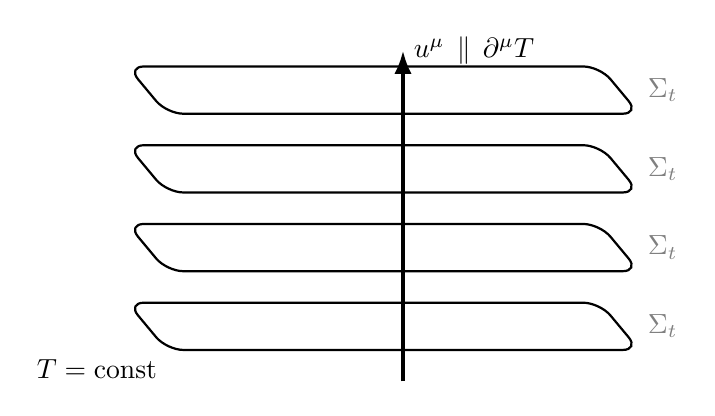
\begin{tikzpicture}[scale=1.0]
\foreach \y in {0,1.0,2.0,3.0}{
    \draw[rounded corners=6pt,thick] (-3,\y) -- (3,\y) -- (2.5,\y+0.6) -- (-3.5,\y+0.6) -- cycle;
    \node[gray] at (3.3,\y+0.3) {$\Sigma_t$};
}
\draw[->,very thick] (0,-0.4) -- (0,3.8) node[right] {$u^\mu \,\parallel\, \partial^\mu T$};
\node[below left] at (-3,0) {$T=\text{const}$};
\end{tikzpicture}
\caption{Preferred foliation by $T(x)$ with unit timelike $u^\mu$ normal to the leaves $\Sigma_t$.}
\end{figure}

\begin{figure}[t]\centering
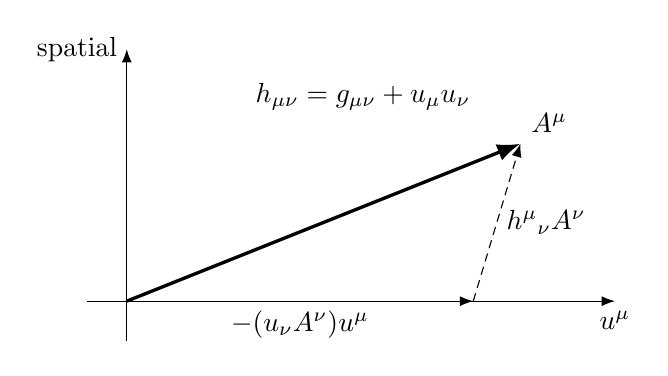
\begin{tikzpicture}[scale=1.0]
\draw[->] (-0.5,0) -- (6.2,0) node[below] {$u^\mu$};
\draw[->] (0,-0.5) -- (0,3.2) node[left] {spatial};
\draw[very thick,->] (0,0) -- (5.0,2.0) node[above right] {$A^\mu$};
\draw[densely dashed,->] (0,0) -- (4.4,0) node[midway,below] {$-(u_\nu A^\nu)u^\mu$};
\draw[densely dashed,->] (4.4,0) -- (5.0,2.0) node[midway,right] {$h^\mu{}_\nu A^\nu$};
\node at (3.0,2.6) {$h_{\mu\nu}=g_{\mu\nu}+u_\mu u_\nu$};
\end{tikzpicture}
\caption{Any vector decomposes into temporal and spatial parts via the projector $h^\mu{}_\nu$.}
\end{figure}

% ============================================================
% 2. Fields & Kinematics
% ============================================================

\begin{figure}[t]\centering
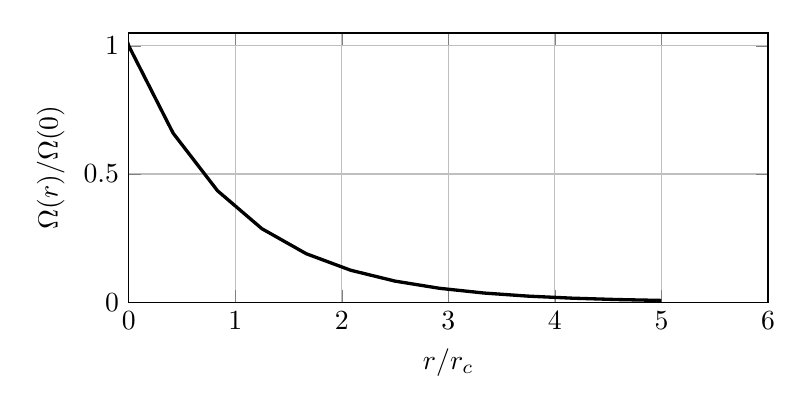
\begin{tikzpicture}
\begin{axis}[width=0.8\linewidth,height=5cm,
xlabel={$r/r_c$}, ylabel={$\Omega(r)/\Omega(0)$},
xmin=0,xmax=6, ymin=0, ymax=1.05, grid=both]
\addplot[very thick] {exp(-x)};
\end{axis}
\end{tikzpicture}
\caption{Canonical profile $\Omega(r)=\Omega(0)e^{-r/r_c}$.}
\end{figure}

\begin{figure}[t]\centering
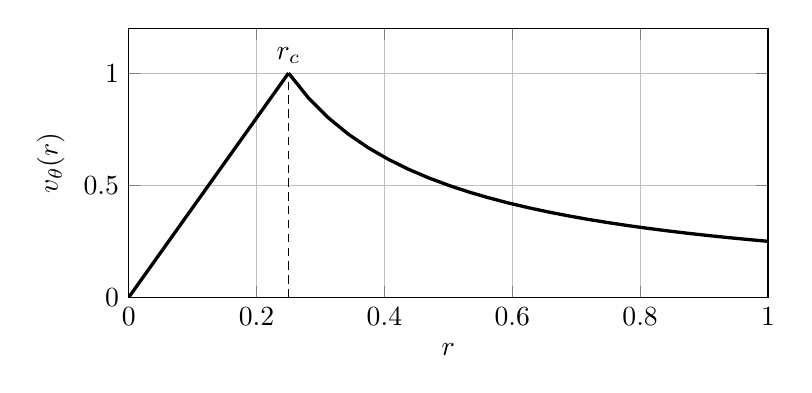
\begin{tikzpicture}
\begin{axis}[width=0.8\linewidth,height=5cm,
xlabel={$r$}, ylabel={$v_\theta(r)$}, xmin=0,xmax=1, ymin=0,ymax=1.2, grid=both]
\addplot[very thick,domain=0:0.25] {4*x};           % rigid core
\addplot[very thick,domain=0.25:1]  {1.0/(4*x)};     % irrotational
\draw[densely dashed] (0.25,0) -- (0.25,1) node[above] {$r_c$};
\end{axis}
\end{tikzpicture}
\caption{Rankine model: solid‐body core ($v\propto r$) matched to irrotational shell ($v\propto 1/r$).}
\end{figure}

% ============================================================
% 3. Action & Couplings
% ============================================================

\begin{figure}[t]\centering
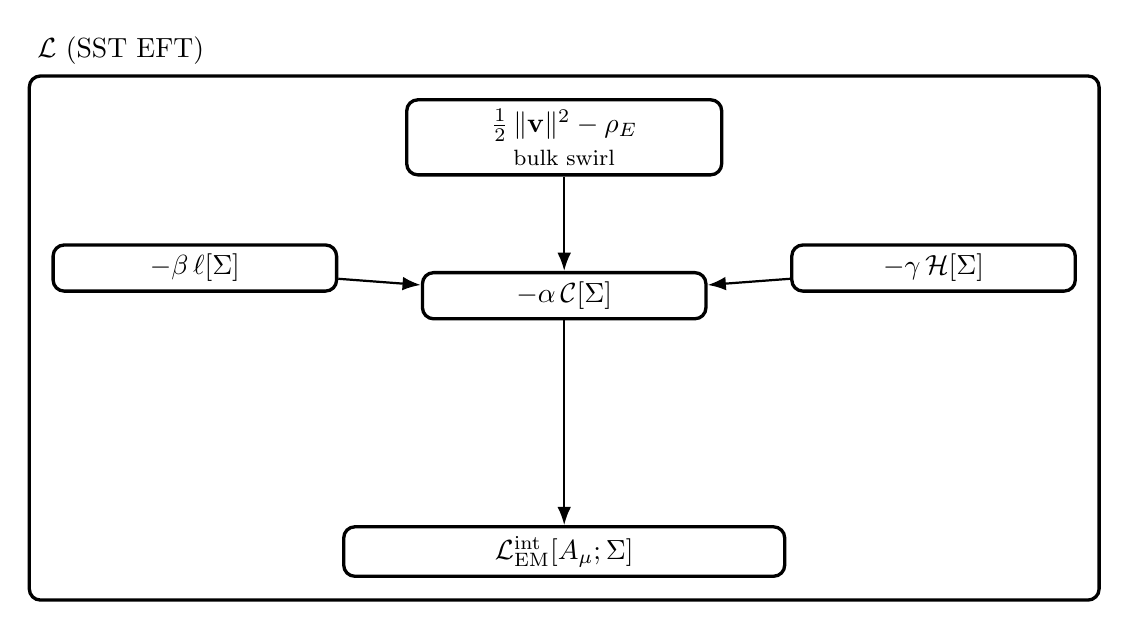
\begin{tikzpicture}[node distance=1.2cm]
\node[draw,rounded corners,very thick,align=center,minimum width=4cm] (bulk) {$\tfrac12\rhof\,\|\mathbf v\|^2-\rho_E$\\\footnotesize bulk swirl};
\node[draw,rounded corners,very thick,below left=of bulk,align=center,minimum width=3.6cm] (len) {$-\beta\,\ell[\Sigma]$};
\node[draw,rounded corners,very thick,below=of bulk,align=center,minimum width=3.6cm] (cont) {$-\alpha\,\mathcal C[\Sigma]$};
\node[draw,rounded corners,very thick,below right=of bulk,align=center,minimum width=3.6cm] (hel) {$-\gamma\,\mathcal H[\Sigma]$};
\node[draw,rounded corners,very thick,below=2.6cm of cont,align=center,minimum width=5.6cm] (em) {$\mathcal L_{\rm EM}^{\rm int}[A_\mu;\Sigma]$};
\draw[->,thick] (bulk) -- (cont);
\draw[->,thick] (len) -- (cont);
\draw[->,thick] (hel) -- (cont);
\draw[->,thick] (cont) -- (em);
\node[draw,rounded corners,very thick,fit=(bulk)(len)(cont)(hel)(em),inner sep=8pt] (box) {};
\node[above right] at (box.north west) {$\mathcal L$ (SST EFT)};
\end{tikzpicture}
\caption{SST Lagrangian as modular terms.}
\end{figure}

\begin{figure}[t]\centering
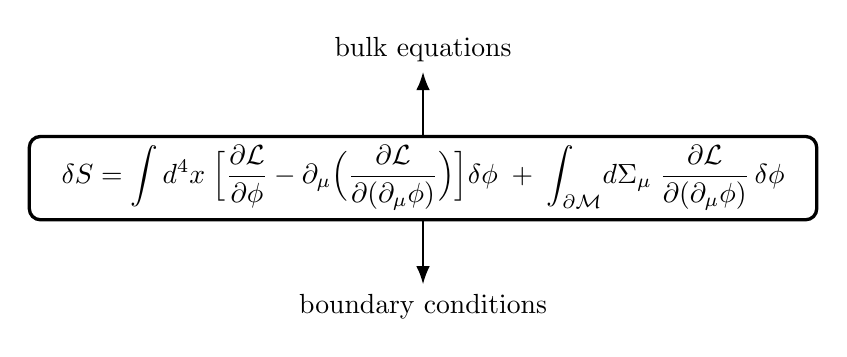
\begin{tikzpicture}[scale=1.0]
\node[draw,rounded corners,very thick,align=left,minimum width=10cm] (EL)
{$\displaystyle \delta S=\int d^4x\;\Big[\frac{\partial \mathcal L}{\partial \phi}-\partial_\mu\Big(\frac{\partial \mathcal L}{\partial(\partial_\mu\phi)}\Big)\Big]\delta\phi\;+\;\int_{\partial\mathcal M}\! d\Sigma_\mu \;\frac{\partial \mathcal L}{\partial(\partial_\mu\phi)}\,\delta\phi$};
\draw[->,thick] (EL.north) -- ++(0,0.8) node[above] {bulk equations};
\draw[->,thick] (EL.south) -- ++(0,-0.8) node[below] {boundary conditions};
\end{tikzpicture}
\caption{Variation of the action: Euler–Lagrange equations plus boundary term.}
\end{figure}

% ============================================================
% 4. Linearized Modes & Constraints
% ============================================================

\begin{figure}[t]\centering
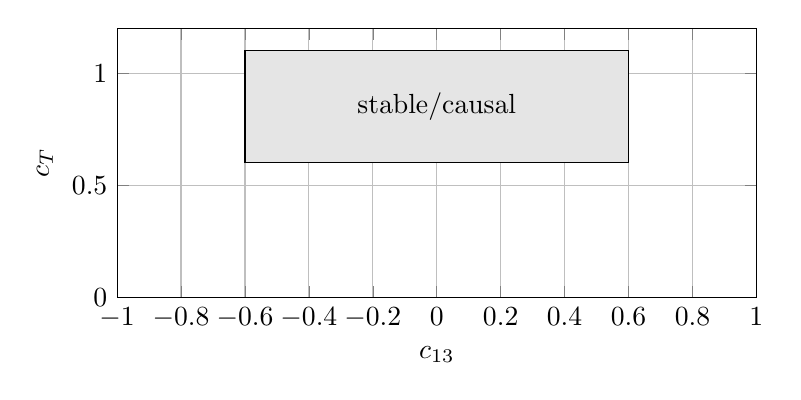
\begin{tikzpicture}
\begin{axis}[width=0.8\linewidth,height=5cm,
xlabel={$c_{13}$}, ylabel={$c_T$}, xmin=-1,xmax=1, ymin=0,ymax=1.2, grid=both]
\addplot[fill=black!10,draw=black] coordinates {
    (-0.6,0.6) (0.6,0.6) (0.6,1.1) (-0.6,1.1) } -- cycle;
\node at (axis cs:0,0.85) {stable/causal};
\end{axis}
\end{tikzpicture}
\caption{Illustrative stability/causality window in $(c_{13},c_T)$.}
\end{figure}

\begin{figure}[t]\centering
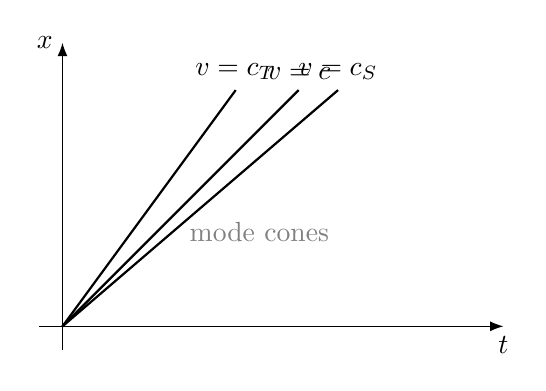
\begin{tikzpicture}[scale=1.0]
\draw[->] (-0.3,0) -- (5.6,0) node[below] {$t$};
\draw[->] (0,-0.3) -- (0,3.6) node[left] {$x$};
\draw[thick] (0,0) -- (3,3) node[above] {$v=c$};
\draw[thick] (0,0) -- (2.2,3) node[above] {$v=c_T$};
\draw[thick] (0,0) -- (3.5,3) node[above] {$v=c_S$};
\node[gray] at (2.5,1.2) {mode cones};
\end{tikzpicture}
\caption{Linearized mode cones with different propagation speeds.}
\end{figure}

% ============================================================
% 5. Strings / Worldsheet Coupling
% ============================================================

\begin{figure}[t]\centering
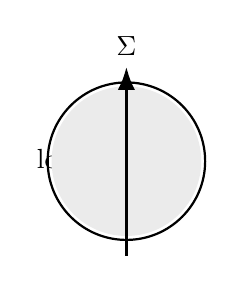
\begin{tikzpicture}[scale=1.0]
\draw[thick] (-2,0) circle (1.0) node[left=10pt] {loop};
\fill[black!8] (-2,0) circle (0.95);
\draw[->,very thick] (-2,-1.2) -- (-2,1.2) node[above] {$\Sigma$};
\end{tikzpicture}
\caption{String loop and its worldsheet $\Sigma$ (schematic).}
\end{figure}

\begin{figure}[t]\centering
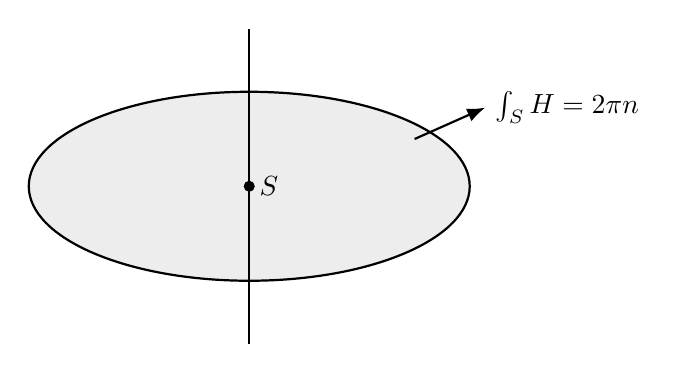
\begin{tikzpicture}[scale=1.0]
\fill[black!7] (0,0) ellipse (2.8 and 1.2);
\draw[thick] (0,0) ellipse (2.8 and 1.2) node[right] {$S$};
\draw[thick] (0,-2) -- (0,2);
\fill (0,0) circle (2pt);
\draw[->,thick] (2.1,0.6) -- ++(0.9,0.4) node[right] {$\int_S H=2\pi n$};
\end{tikzpicture}
\caption{Worldsheet piercing a surface $S$, quantizing the $H$-flux.}
\end{figure}

% ============================================================
% 6. Conservation Laws
% ============================================================

\begin{figure}[t]\centering
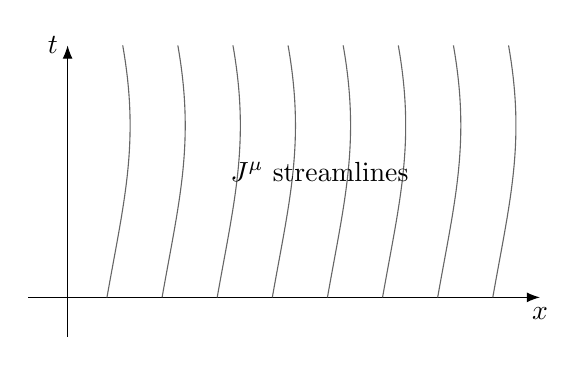
\begin{tikzpicture}[scale=1.0]
\draw[->] (-0.5,0) -- (6,0) node[below] {$x$};
\draw[->] (0,-0.5) -- (0,3.2) node[left] {$t$};
\foreach \x in {0.5,1.2,...,5.5}{
    \draw[black!60] (\x,0) to[out=80,in=-80] (\x+0.2,3.2);
}
\node at (3.2,1.6) {$J^\mu$ streamlines};
\end{tikzpicture}
\caption{Schematic Noether current $J^\mu$ flowlines.}
\end{figure}

\begin{figure}[t]\centering
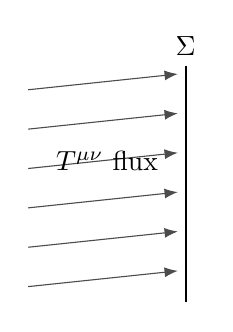
\begin{tikzpicture}[scale=1.0]
\draw[thick] (0,0) -- (0,3) node[above] {$\Sigma$};
\foreach \y in {0.2,0.7,...,2.7}{
    \draw[->,black!70] (-2,\y) -- (-0.1,\y+0.2);
}
\node at (-1.0,1.8) {$T^{\mu\nu}$ flux};
\end{tikzpicture}
\caption{Energy–momentum flux crossing a surface element.}
\end{figure}

% ============================================================
% 7. Canon Profiles & Pressure Well
% ============================================================

\begin{figure}[t]\centering
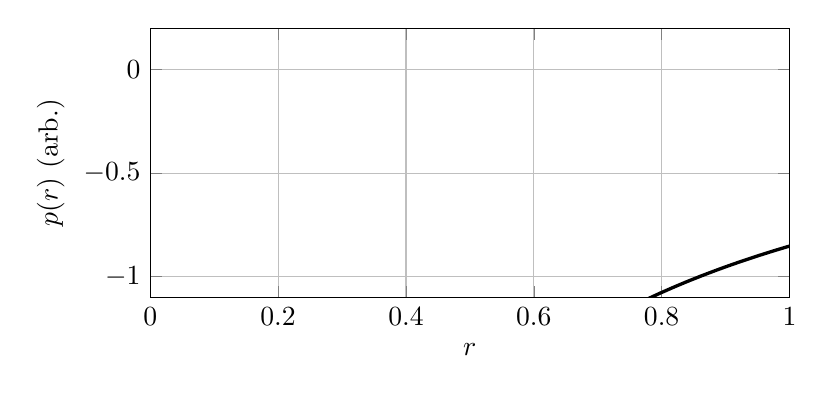
\begin{tikzpicture}
\begin{axis}[width=0.8\linewidth,height=5cm,
xlabel={$r$}, ylabel={$p(r)$ (arb.)}, xmin=0,xmax=1, ymin=-1.1,ymax=0.2, grid=both]
\addplot[very thick,domain=0.02:1,samples=200] {-1.0/(x+0.05) + 0.1};
\end{axis}
\end{tikzpicture}
\caption{Qualitative pressure well induced by swirl.}
\end{figure}

\begin{figure}[t]\centering
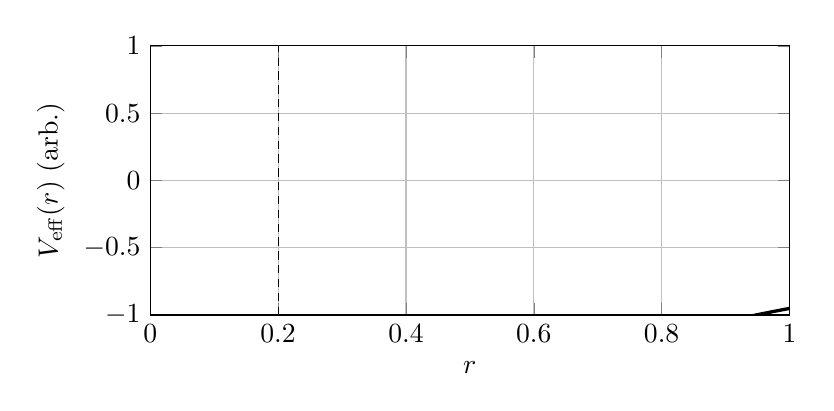
\begin{tikzpicture}
\begin{axis}[width=0.8\linewidth,height=5cm,
xlabel={$r$}, ylabel={$V_{\rm eff}(r)$ (arb.)}, xmin=0,xmax=1, ymin=-1.0,ymax=1.0, grid=both]
\addplot[very thick,domain=0.05:1,samples=200] {-1/(x+0.05) + 0.6*exp(-10*(x-0.2)^2)};
\draw[densely dashed] (0.2,-1.0) -- (0.2,1.0) node[above] {$r_c$};
\end{axis}
\end{tikzpicture}
\caption{Effective potential with core scale $r_c$ (schematic).}
\end{figure}

% ============================================================
% 8. Parameter Space / Sensitivity
% ============================================================

\begin{figure}[t]\centering
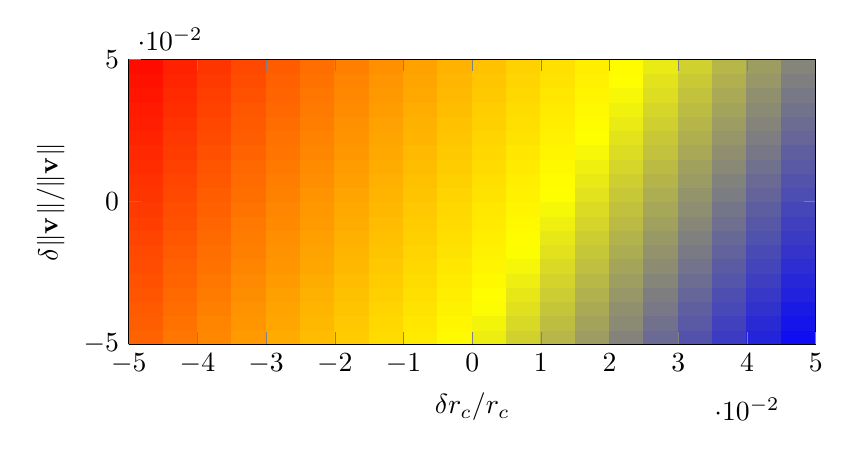
\begin{tikzpicture}
\begin{axis}[width=0.85\linewidth,height=5.2cm,
view={0}{90}, xlabel={$\delta r_c/r_c$}, ylabel={$\delta \|\mathbf v_{\circlearrowleft}\|/\|\mathbf v_{\circlearrowleft}\|$}]
\addplot3[surf,shader=flat,mesh/ordering=y varies,point meta=z, samples=21,domain=-0.05:0.05,y domain=-0.05:0.05]
    {(1 + y)*1/(1 + 2*x)^2 - 1};
\end{axis}
\end{tikzpicture}
\caption{Illustrative relative change $\delta G/G$ vs.\ small parameter shifts (toy scaling).}
\end{figure}

\begin{figure}[t]\centering
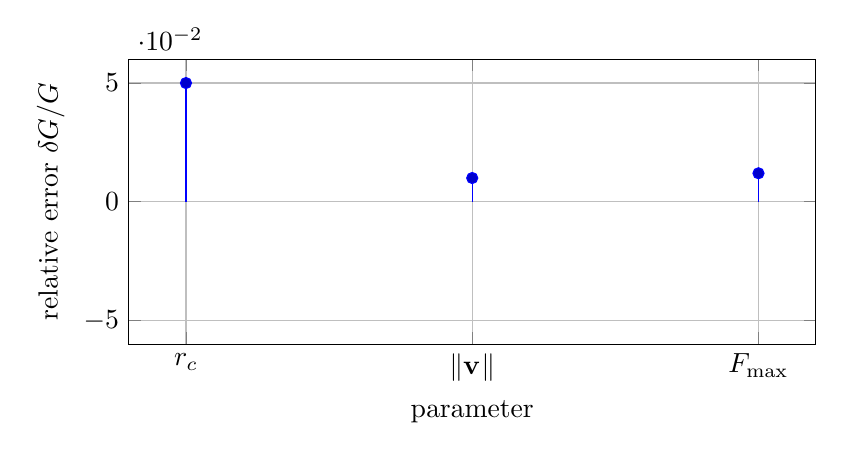
\begin{tikzpicture}
\begin{axis}[width=0.85\linewidth,height=5.2cm,
xlabel={parameter}, ylabel={relative error $\delta G/G$},
xtick={1,2,3}, xticklabels={$r_c$, $\|\mathbf v_{\circlearrowleft}\|$, $F_{\max}$},
ymin=-0.06, ymax=0.06, grid=both]
\addplot+[ycomb,mark=*] coordinates {(1,0.05) (2,0.01) (3,0.012)};
\end{axis}
\end{tikzpicture}
\caption{Toy sensitivity bars (edit with actual derivatives).}
\end{figure}



\begin{figure}[t]
\centering
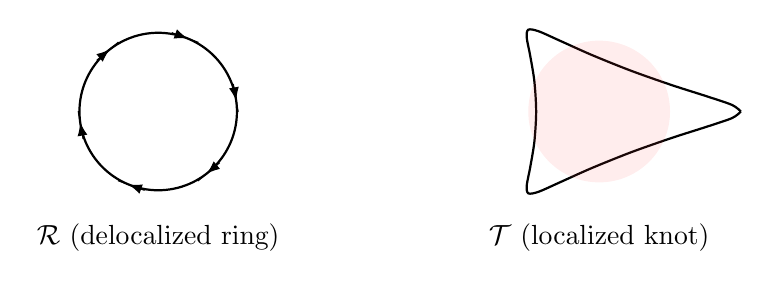
\begin{tikzpicture}[scale=1,>=Latex,decoration={markings,mark=at position 0.6 with {\arrow{>}}}]
    % Left: ring R
\draw[thick] (-3,0) circle (1);
\foreach \a in {10,70,130,190,250,310}{
    \draw[postaction={decorate}] (-3,0) ++({cos(\a)},{sin(\a)}) ++({-0.18*sin(\a)},{0.18*cos(\a)}) -- ++({0.36*sin(\a)},{-0.36*cos(\a)});
}
\node[below] at (-3,-1.3) {$\mathcal R$ (delocalized ring)};

% Right: trefoil T (schematic)
\draw[thick,domain=0:360,smooth,variable=\t]
plot ({2.6+1.3*cos(\t)+0.5*cos(2*\t)},{0.0+0.9*sin(\t)-0.3*sin(2*\t)});
\fill[red!70,opacity=0.1] (2.6,0) circle (0.9);
\node[below] at (2.6,-1.3) {$\mathcal T$ (localized knot)};
\end{tikzpicture}
\caption{Two-phase electron in SST: delocalized toroidal circulation $\mathcal R$ and localized knotted soliton $\mathcal T$.}
\end{figure}
2) Circulation quantization on a ring
latex
Copy code
\begin{figure}[t]
\centering
\begin{tikzpicture}[scale=1.1,>=Latex]
\draw[thick] (0,0) circle (2);
% Tangential arrows
\foreach \a in {0,40,...,320}{
    \draw[->,very thick] (2*cos(\a),2*sin(\a)) -- ++({0.5*sin(\a)},{-0.5*cos(\a)});
}
% Phase ticks
\foreach \a in {0,60,...,300}{
    \draw[line width=1pt] ({1.8*cos(\a)},{1.8*sin(\a)}) -- ({2.2*cos(\a)},{2.2*sin(\a)});
}
\node at (0,-2.8) {$\Gamma_n=\oint v\!\cdot d\ell = n\frac{h}{m_e}, \quad \lambda_{\rm ring}=\frac{2\pi R}{n}=\frac{h}{p_\theta}$};
\end{tikzpicture}
\caption{Circulation quantization and de Broglie relation on the ring phase $\mathcal R$.}
\end{figure}
3) Energy landscape for
𝑅
→
𝑇
R→T
latex
Copy code
\begin{figure}[t]
\centering
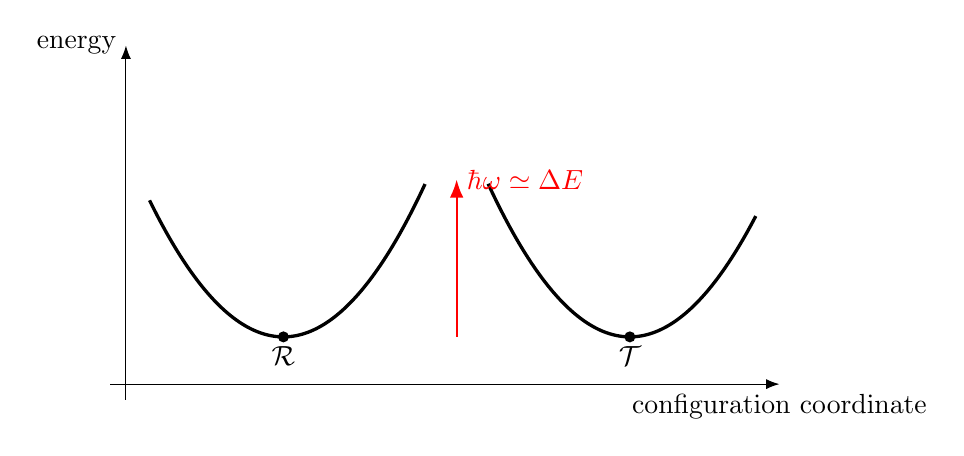
\begin{tikzpicture}[scale=1.0,>=Latex]
    % Axes
\draw[->] (-0.2,0) -- (8.3,0) node[below] {configuration coordinate};
\draw[->] (0,-0.2) -- (0,4.3) node[left] {energy};
% Double-well (piecewise smooth)
\draw[very thick,domain=0.3:3.8,samples=100] plot(\x,{0.6*(\x-2)^2+0.6});
\draw[very thick,domain=4.6:8.0,samples=100] plot(\x,{0.6*(\x-6.4)^2+0.6});
% Minima points
\fill (2,0.6) circle (2pt) node[below] {$\mathcal R$};
\fill (6.4,0.6) circle (2pt) node[below] {$\mathcal T$};
% Vertical resonance arrow
\draw[->,red,thick] (4.2,0.6) -- ++(0,2) node[right] {$\hbar\omega \simeq \Delta E$};
\end{tikzpicture}
\caption{SST transition energy: $\Delta E=(\epsilon_0A+\beta)\Delta L+\alpha C(\mathcal T)+\gamma\mathcal H(\mathcal T)$.}
\end{figure}
4) Preferred foliation and
𝑢
𝜇
u
μ

latex
Copy code
\begin{figure}[t]
\centering
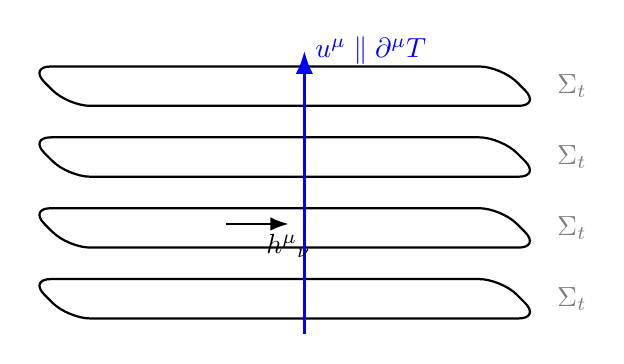
\begin{tikzpicture}[scale=1.0,>=Latex]
    % Stacked leaves
\foreach \y in {0,0.9,1.8,2.7}{
    \draw[rounded corners=8pt,thick] (-3,\y) -- (3,\y) -- (2.5,\y+0.5) -- (-3.5,\y+0.5) -- cycle;
    \node[gray] at (3.4,\y+0.25) {$\Sigma_{t}$};
}
% Foliation vector u
\draw[->,very thick,blue] (0,-0.2) -- (0,3.4) node[right] {$u^\mu \parallel \partial^\mu T$};
% Projection hint
\draw[->,thick] (-1,1.2) -- (-0.2,1.2) node[below] {$h^\mu{}_\nu$};
\end{tikzpicture}
\caption{Preferred foliation by the clock field $T(x)$ with unit timelike $u^\mu$, and spatial projector $h_{\mu\nu}=g_{\mu\nu}+u_\mu u_\nu$.}
\end{figure}
5) Flux of
𝐻
=
d
𝐵
H=dB through a surface pierced by a string
latex
Copy code
\begin{figure}[t]
\centering
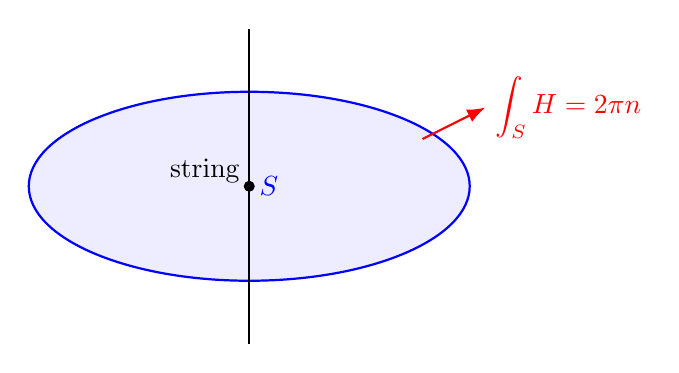
\begin{tikzpicture}[scale=1.0,>=Latex]
    % Surface
\fill[blue!7] (0,0) ellipse (2.8 and 1.2);
\draw[thick,blue] (0,0) ellipse (2.8 and 1.2) node[right] {$S$};
% String piercing
\draw[thick] (0,-2) -- (0,2);
\fill (0,0) circle (2pt);
\node[left] at (0,0.2) {string};
% Flux arrow
\draw[->,red,thick] (2.2,0.6) -- ++(0.8,0.4) node[right] {$\displaystyle \int_S H=2\pi n$};
\end{tikzpicture}
\caption{Worldsheet/flux cartoon: the swirl string pierces $S$, quantizing the $H$-flux.}
\end{figure}



\section*{1) Mach–Zehnder Interferometer (SST view)}




\begin{figure}[t]
\centering
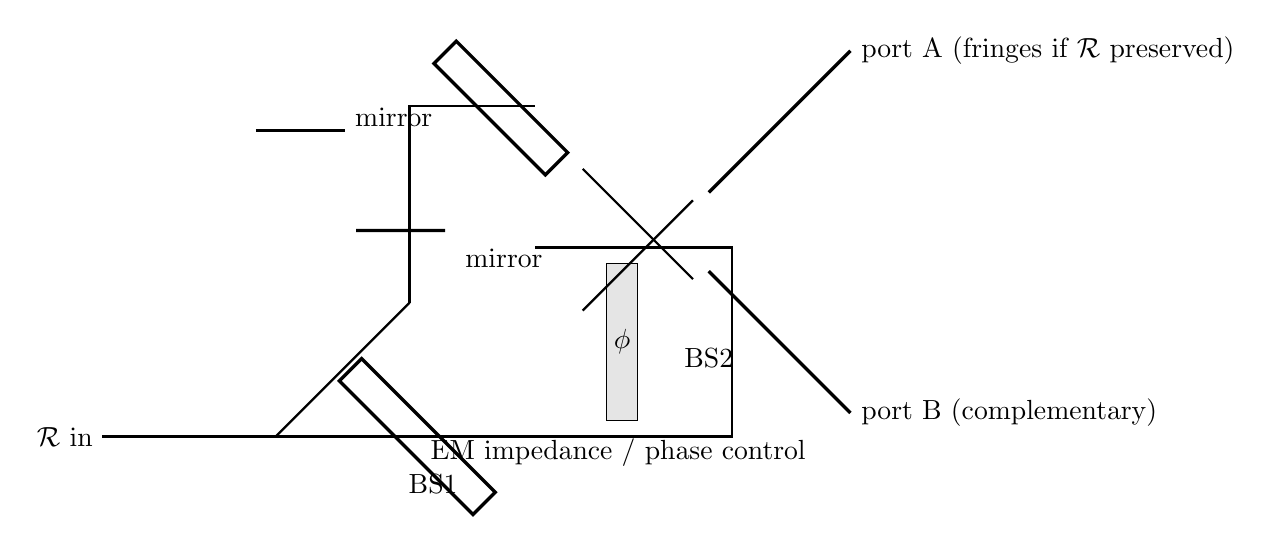
\begin{tikzpicture}[scale=1.0]
  % Components
  \draw[very thick] (-4,0) -- (-1.8,0); % input
  \node[left] at (-4,0) {$\mathcal R$ in};
  % BS1
  \draw[very thick,rotate=45] (-0.2,-1.2) rectangle (0.2,1.2);
  % Paths
  \draw[thick] (-1.8,0) -- (-0.1,1.7);    % up-left to BS1
  \draw[thick] (-1.8,0) -- (1.7,0);       % straight to BS1
  % After BS1 (split)
  \draw[thick] (1.7,0) -- (4.0,0) -- (4.0,2.4) -- (1.5,2.4); % upper arm to mirror
  \draw[thick] (-0.1,1.7) -- (-0.1,4.2) -- (1.5,4.2);        % lower arm up to mirror
  % Phase plate in upper arm
  \draw[fill=black!10,draw=black] (2.4,0.2) rectangle (2.8,2.2);
  \node at (2.6,1.2) {$\phi$};
  % Mirrors
  \draw[very thick,rotate=45] (1.3,2.4) -- (2.1,1.6);
  \draw[very thick,rotate=45] (1.3,4.2) -- (2.1,3.4);
  % Recombine at BS2
  \draw[thick] (2.1,1.6) -- (3.5,3.0); % to BS2
  \draw[thick] (2.1,3.4) -- (3.5,2.0); % to BS2
  \draw[very thick,rotate=45] (3.5,1.2) rectangle (3.9,3.2); % BS2
  % Outputs
  \draw[very thick] (3.7,3.1) -- (5.5,4.9) node[right] {port A (fringes if $\mathcal R$ preserved)};
  \draw[very thick] (3.7,2.1) -- (5.5,0.3) node[right] {port B (complementary)};
  % Labels
  \node[below] at (2.55,0.1) {EM impedance / phase control};
  \node[below] at (-0.3,4.3) {mirror};
  \node[below] at (1.1,2.5) {mirror};
  \node at (0.2,-0.6) {BS1};
  \node at (3.7,1.0) {BS2};
\end{tikzpicture}
\caption{Mach–Zehnder in SST. The delocalized $\mathcal R$ phase splits/recombines; a phase/impedance element $\phi$ controls output fringes vs.\ which-way collapse to $\mathcal T$.}
\end{figure}




\section*{2) Knot invariants overlay on a trefoil (C(K)C(K)C(K), H(K)\mathcal H(K)H(K))}




\begin{figure}[t]
\centering
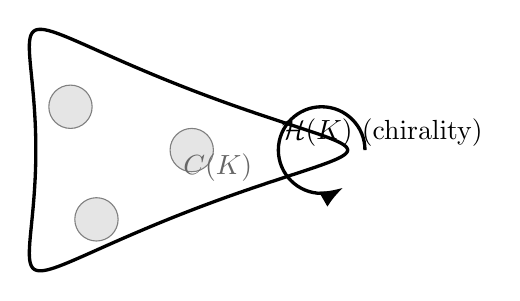
\begin{tikzpicture}[scale=1.1]
  % Trefoil (planar schematic)
  \draw[very thick,domain=0:360,samples=400,smooth,variable=\t]
    plot ({1.8*cos(\t)+0.6*cos(2*\t)},{1.2*sin(\t)-0.4*sin(2*\t)});
  % Near-contact disks (proxy for C(K))
  \foreach \P in {(0.6,0.0),(-0.8,0.5),(-0.5,-0.8)}{
    \draw[black!50,fill=black!10] \P circle (0.25);
  }
  \node[black!60] at (0.9,-0.2) {$C(K)$};
  % Helicity arrow/glyph
  \draw[->,very thick] (2.6,0.0) arc (0:300:0.5);
  \node at (2.8,0.2) {$\mathcal H(K)$ (chirality)};
\end{tikzpicture}
\caption{Trefoil schematic with overlays indicating near-contact regions ($C(K)$) and helicity/chirality cue ($\mathcal H(K)$).}
\end{figure}




\section*{3) Core profile Ω(r)\Omega(r)Ω(r) and Swirl Clock dtlocal/dt∞dt_{\rm local}/dt_\inftydtlocal​/dt∞​}




\begin{figure}[t]
\centering
\begin{minipage}{0.47\linewidth}
\centering
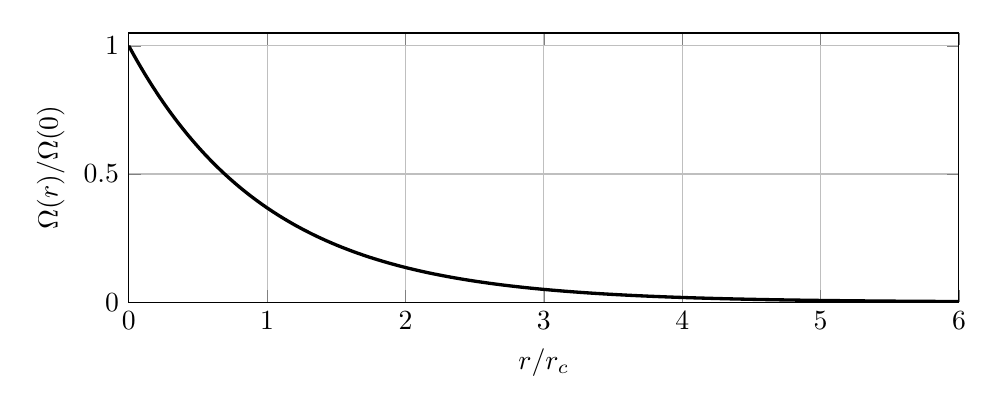
\begin{tikzpicture}
\begin{axis}[
  width=\linewidth,height=5cm,
  xlabel={$r/r_c$}, ylabel={$\Omega(r)/\Omega(0)$},
  xmin=0,xmax=6, ymin=0, ymax=1.05,
  domain=0:6, samples=200, grid=both]
\addplot[very thick] {exp(-x)};
\end{axis}
\end{tikzpicture}
\caption*{\(\Omega(r)=\Omega(0)e^{-r/r_c}\).}
\end{minipage}\hfill
\begin{minipage}{0.47\linewidth}
\centering
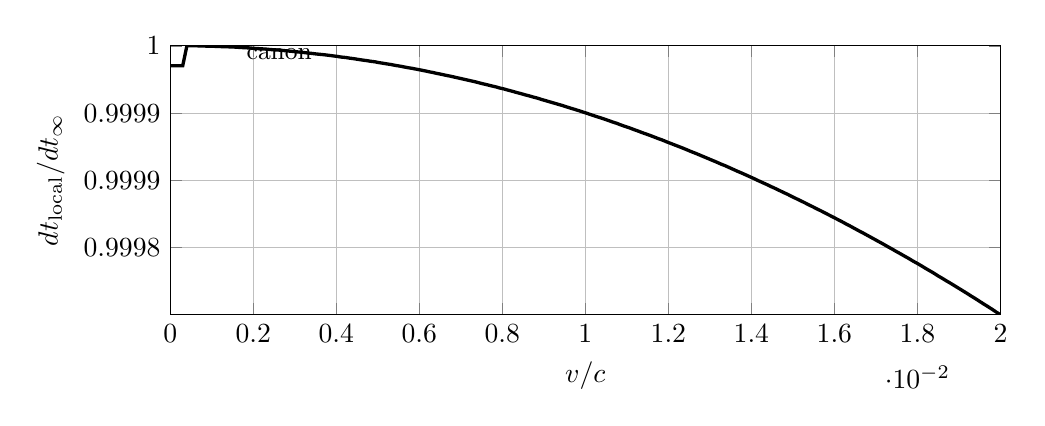
\begin{tikzpicture}
\begin{axis}[
  width=\linewidth,height=5cm,
  xlabel={$v/c$}, ylabel={$dt_{\rm local}/dt_\infty$},
  xmin=0,xmax=0.02, ymin=0.9998, ymax=1.0000,
  grid=both, yticklabel style={/pgf/number format/fixed, /pgf/number format/precision=4}]
\addplot[very thick,domain=0:0.02,samples=200] {sqrt(1 - x^2)};
\addplot[densely dashed] coordinates {(0.00365,0.9999933)} node[pos=0, left] {\small canon};
\end{axis}
\end{tikzpicture}
\caption*{Swirl Clock: \(\sqrt{1-v^2/c^2}\), with canonical point marked.}
\end{minipage}
\caption{Left: canonical angular profile. Right: local time rate vs.\ \(v/c\).}
\end{figure}




\section*{4) Fringe geometry (slit separation sss, distance LLL, screen coordinate xxx)}




\begin{figure}[t]
\centering
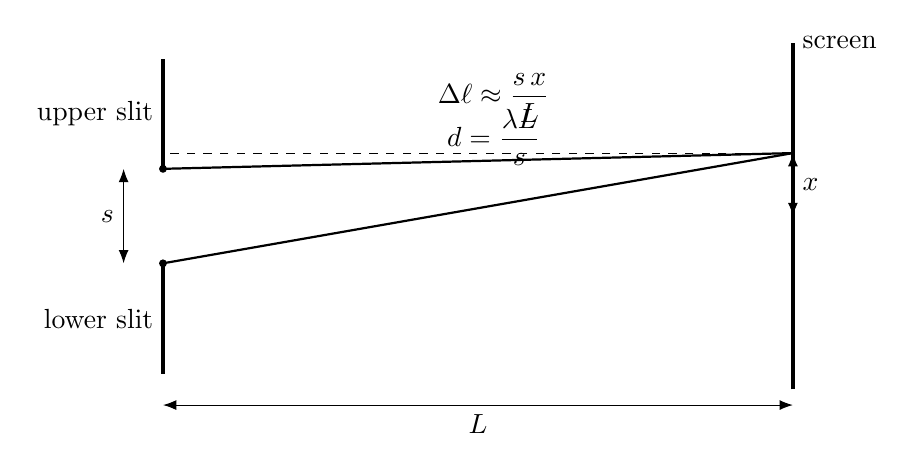
\begin{tikzpicture}[scale=1.0]
  % Slits
  \draw[very thick] (0,-2) -- (0,-0.6);
  \draw[very thick] (0, 0.6) -- (0, 2.0);
  \fill (0, 0.6) circle (0.05);
  \fill (0,-0.6) circle (0.05);
  \node[left] at (0,1.3) {upper slit};
  \node[left] at (0,-1.3) {lower slit};
  \draw[<->] (-0.5,0.6) -- (-0.5,-0.6) node[midway,left] {$s$};

  % Screen
  \draw[very thick] (8,-2.2) -- (8,2.2);
  \node[right] at (8,2.2) {screen};
  % Point x on screen
  \draw[dashed] (8,0.8) -- (0,0.8);
  \draw[<->] (8,0) -- (8,0.8) node[midway,right] {$x$};
  % Distance L
  \draw[<->] (0,-2.4) -- (8,-2.4) node[midway,below] {$L$};

  % Rays from slits to point
  \draw[thick] (0,0.6) -- (8,0.8);
  \draw[thick] (0,-0.6) -- (8,0.8);

  % Path difference annotation
  \node at (4.2,1.5) {$\Delta \ell \approx \dfrac{s\,x}{L}$};
  \node at (4.2,1.0) {$d=\dfrac{\lambda L}{s}$};
\end{tikzpicture}
\caption{Double-slit geometry: path difference \(\Delta \ell \approx s\,x/L\) and fringe spacing \(d=\lambda L/s\).}
\end{figure}




\section*{5) Polarization selection (helicity matching to trefoil chirality)}




\begin{figure}[t]
\centering
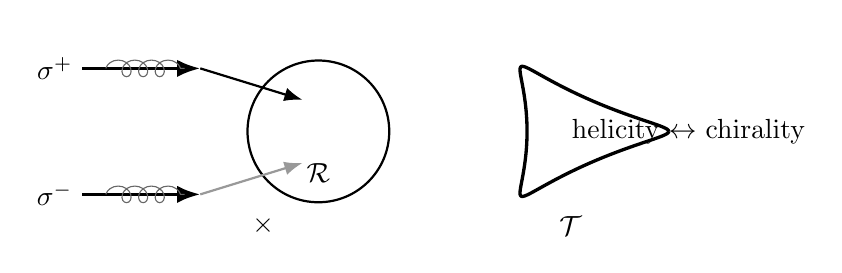
\begin{tikzpicture}[scale=1.0]
  % Left: CP- light symbols
  \draw[very thick,->] (-3,0.8) -- (-1.5,0.8);
  \draw[very thick,->] (-3,-0.8) -- (-1.5,-0.8);
  \node[left] at (-3,0.8) {$\sigma^+$};
  \node[left] at (-3,-0.8) {$\sigma^-$};
  \draw[black!60,decorate,decoration={coil,aspect=1,segment length=6pt,amplitude=3pt}] (-2.7,0.8) -- (-1.7,0.8);
  \draw[black!60,decorate,decoration={coil,aspect=1,segment length=6pt,amplitude=3pt}] (-2.7,-0.8) -- (-1.7,-0.8);

  % Center: ring and trefoil
  \draw[thick] (0,0) circle (0.9) node[below=8pt] {$\mathcal R$};
  \draw[very thick,domain=0:360,samples=200,smooth,variable=\t]
    plot ({3.2+0.9*cos(\t)+0.35*cos(2*\t)},{0.0+0.7*sin(\t)-0.25*sin(2*\t)});
  \node at (3.2,-1.2) {$\mathcal T$};

  % Matching/mismatch markers
  \node at (-0.7,1.2) {$\checkmark$};
  \node at (-0.7,-1.2) {$\times$};
  \node at (4.7,0.0) {helicity $\leftrightarrow$ chirality};

  % Arrows showing coupling strength conceptually
  \draw[->,thick] (-1.5,0.8) -- (-0.2,0.4);
  \draw[->,thick,black!40] (-1.5,-0.8) -- (-0.2,-0.4);
\end{tikzpicture}
\caption{Helicity selection: circularly polarized light \(\sigma^\pm\) couples preferentially to the chirality of the target knot \(\mathcal T\), setting transition strength.}
\end{figure}




\section*{6) (Already supplied earlier) Visibility vs.\ which-way coupling V=e−Γτ\mathcal V=e^{-\Gamma\tau}V=e−Γτ}

\textit{(Keep for completeness; no changes needed.)}



\section*{7) (Optional EFT block diagram) Lagrangian terms as modules}




\begin{figure}[t]
\centering
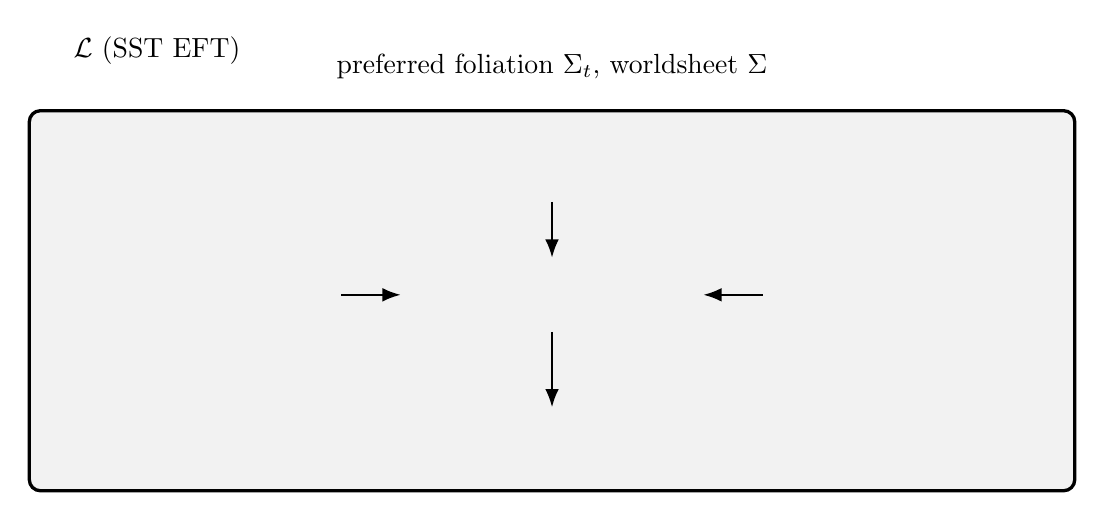
\begin{tikzpicture}[scale=1.0]
  \node[draw,very thick,rounded corners,align=center,minimum width=4.2cm,minimum height=1.0cm] (bulk)
    at (0,1.5) {$\tfrac12\rhof\,\|\mathbf v\|^2 - \rho_E$ \\ bulk swirl};
  \node[draw,very thick,rounded corners,minimum width=3.8cm,minimum height=0.9cm] (len)
    at (-4.6,-0.2) {$-\beta\,\ell[\Sigma]$};
  \node[draw,very thick,rounded corners,minimum width=3.8cm,minimum height=0.9cm] (cont)
    at (0,-0.2) {$-\alpha\,\mathcal C[\Sigma]$};
  \node[draw,very thick,rounded corners,minimum width=3.8cm,minimum height=0.9cm] (hel)
    at (4.6,-0.2) {$-\gamma\,\mathcal H[\Sigma]$};
  \node[draw,very thick,rounded corners,minimum width=5.4cm,minimum height=0.9cm] (em)
    at (0,-2.1) {$\mathcal L_{\rm EM}^{\rm int}[A_\mu;\Sigma]$};

  \node[draw,very thick,rounded corners,fill=black!5,minimum width=12cm,minimum height=4.8cm,fit=(bulk)(len)(cont)(hel)(em)] (L) {};
  \node[above right] at (-6.2,2.6) {$\displaystyle \mathcal L$ (SST EFT)};

  \draw[->,thick] (bulk) -- (cont);
  \draw[->,thick] (len) -- (cont);
  \draw[->,thick] (hel) -- (cont);
  \draw[->,thick] (cont) -- (em);

  \node at (0,2.7) {preferred foliation \(\Sigma_t\), worldsheet \(\Sigma\)};
\end{tikzpicture}
\caption{SST EFT ingredients as modular terms composing \(\mathcal L\).}
\end{figure}



\end{document}